\clearpage
\subsection{Historically exposed full-DFT functional pilot}
A separate, zero-offset ROKS comparison uses PBE0, CAM-B3LYP and
$\omega$B97X\cite{Chai2008WB97X} at the same fixed geometries and spherical
aug-cc-pVDZ basis (grid level 3). Four pilot targets select one global
functional by MAE; acetaldehyde and acetone are the reserved confirmation
targets for this selection. All six labels had been exposed historically,
so this is not blind validation. The QUEST targets use TBE/AVTZ values;
the smaller calculation basis has not been extrapolated. No semiempirical
kernel scale or energy offset enters these calculations.

All 18 functional/state calculations pass the $10^{-8}$ orbital-residual
criterion and frozen hole/particle overlaps of at least 0.7. Alternative
stationary roots are retained separately. Deterministic continuation
transfers only orbitals from an already qualified functional; the final
energy and complete response use the requested functional. Archived
Cartesian AO references are projected into the common spherical basis
after checking their checkpoint metric and geometry.

\begin{table}[htbp]
\centering\small
\caption{Full-DFT common-orbital ROKS vertical energies (eV). The first four
rows form the pilot; the last two form the confirmation subset.}
\begin{tabular}{lrrrr}
\toprule
Molecule & Reference & PBE0 & CAM-B3LYP & $\omega$B97X \\
\midrule
Formaldehyde & 3.966 & 3.628 & 3.680 & 3.811 \\
Ethylene & 7.897 & 7.087 & 7.162 & 7.421 \\
Butadiene & 6.222 & 5.134 & 5.458 & 5.785 \\
Furan & 6.530 & 7.156 & 7.386 & 7.651 \\
Acetaldehyde & 4.304 & 4.005 & 4.069 & 4.180 \\
Acetone & 4.468 & 4.177 & 4.261 & 4.373 \\
\bottomrule
\end{tabular}
\end{table}

Pilot MAEs are 0.715, 0.660 and 0.547 eV for PBE0, CAM-B3LYP and
$\omega$B97X, respectively, selecting $\omega$B97X. Confirmation MAEs are
0.295, 0.221 and 0.109 eV. The improvement is strongest for the carbonyl
$n\pi^*$ states. It is not uniform across $\pi\pi^*$ states: the furan
error increases to 1.121 eV with $\omega$B97X. Thus this functional is a
candidate for further validation, not a universal accuracy correction.
These results remain separate from the semiempirical 26-state ledger.

\begin{figure}[htbp]
\centering
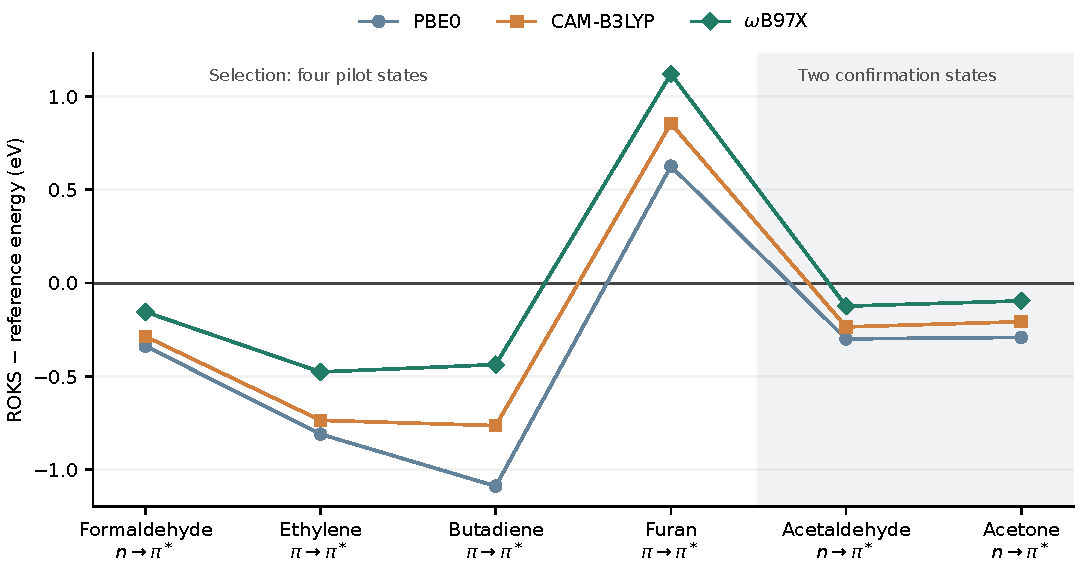
\includegraphics[width=\linewidth]{figures/dft_roks_functional_comparison.pdf}
\caption{Signed full-DFT ROKS errors at fixed geometries, without an energy
offset. Shading marks the two confirmation targets reserved from functional
selection; their labels were nevertheless historically exposed. Lines guide
the eye between distinct molecular targets.}
\end{figure}
